\documentclass{article}

\usepackage{ipprocess}
%\usepackage{lmodern}
%\usepackage{longtable}
\usepackage[latin1]{inputenc} 
\usepackage[T1]{fontenc}
\pagestyle{fancy}
\usepackage{libertine}

%\usepackage[author={Jo�o Carlos Nunes Bittencourt}]{pdfcomment}

\sloppy

\title{32-bit uDLX Core Processor}

\graphicspath{{./pictures/}} % Diret�rio padr�o de figuras.
\makeindex
\begin{document}
  \capa{1.0}{abril}{2014}{32-bit uDLX Core Processor}{Architecture Specification}{Universidade Federal da Bahia}
  \newpage

%%%%%%%%%%%%%%%%%%%%%%%%%%%%%%%%%%%%%%%%%%%%%%%%%%
%% GNU LGPL Licence
%%%%%%%%%%%%%%%%%%%%%%%%%%%%%%%%%%%%%%%%%%%%%%%%%%

  
\begin{center}
\begin{Large}\textbf{GNU LGPL License}                          \end{Large}
\end{center}
\vspace{2cm}
\fbox{
  \parbox{.7\textwidth}{
    \vspace{0,5cm}
    \begin{scriptsize}
    This file is part of uDLX (micro-DeLuX) soft IP-core.\\

    uDLX is free soft IP-core: you can redistribute it and/or modify
    it under the terms of the GNU General Public License as published by
    the Free Software Foundation, either version 3 of the License, or
    (at your option) any later version.\\

    uDLX soft core is distributed in the hope that it will be useful,
    but WITHOUT ANY WARRANTY; without even the implied warranty of
    MERCHANTABILITY or FITNESS FOR A PARTICULAR PURPOSE. See the
    GNU General Public License for more details.

    You should have received a copy of the GNU General Public License
    along with uDLX. If not, see <http://www.gnu.org/licenses/>.
    \end{scriptsize}
    \vspace{0,5cm}
  }
}

\newpage

%%%%%%%%%%%%%%%%%%%%%%%%%%%%%%%%%%%%%%%%%%%%%%%%%%
%% Hist�rico de Revis�es
%%%%%%%%%%%%%%%%%%%%%%%%%%%%%%%%%%%%%%%%%%%%%%%%%%
  \section*{\center Hist�rico de Revis�es}
  \vspace*{1cm}
  \begin{table}[ht] % aqui come�a o ambiente tabela
  \centering
  \begin{tabular}[pos]{|m{2cm} | m{7.2cm} | m{3.8cm}|} 
  \hline % este comando coloca uma linha na tabela
  \cellcolor[gray]{0.9}
  \textbf{Date} & \cellcolor[gray]{0.9}\textbf{Description} & \cellcolor[gray]{0.9}\textbf{Author(s)}\\ \hline
  \hline
  \small 04/14/2014 & \small Conception & \small Jo�o Carlos Bittencourt \\ \hline
  \end{tabular}
  \label{tab:revisoes}
  \end{table}
  
  \newpage
  
  \tableofcontents
  \newpage

%%%%%%%%%%%%%%%%%%%%%%%%%%%%%%%%%%%%%%%%%%%%%%%%%%
%% Concent
%%%%%%%%%%%%%%%%%%%%%%%%%%%%%%%%%%%%%%%%%%%%%%%%%%
  \section{Introduction}
  \subsection{Purpose}
  The main purpose of this document is to define specifications of a uDLX implementation and to provide a full overview of the design. This specifications defines all implementation parameters that composes the general uDLX requirements and specification. This definitions include processor operation modes, instruction set (ISA) and internal registers characteristics. This document also include detailed information of pipeline stages architecture, buses and other supplemental units.
  
  \subsection{Document Outline Description}
  This document is outlined as follow:
	
	\begin{itemize}
	  \item Section : 
	  \item Section : 
	\end{itemize}
		
  \subsection{Acronyms and Abbreviations}
  Along this and other documents part of this project, it will be recurrent the usage of some acronyms and abbreviations. In order to keep track of this elements the Table \ref{tab:definitions} presents a set of abbreviations used and its corresponding meaning.
  
  \FloatBarrier
  \begin{table}[H] % aqui come�a o ambiente tabela
    \begin{center}
      \caption{Acronym and descriptions of elements in this document.}
      \label{tab:definitions}

      \begin{tabular}[pos]{|m{2cm} | m{8cm}|} 
	\hline % este comando coloca uma linha na tabela
	\cellcolor[gray]{0.9}\textbf{Acronym} & \cellcolor[gray]{0.9}\textbf{Description} \\ \hline
	RISC & Reduced Instruction Set Computer \\ \hline
	GPR & General Purpose Registers \\ \hline
	FPGA & Field Gate Programmable Array \\ \hline
	GPPU & General Purpose Processing Unit \\ \hline
	SDRAM & Synchronous Dynamic Random Access Memory\\ \hline
	HDL & Hardware Description Language \\ \hline
	RAW & Read After Write \\ \hline
	CPU & Central Processing Unit \\ \hline
	ISA & Instruction Set Architecture \\ \hline
	ALU & Arithmetic and Logic Unit \\ \hline
	PC  & Program Counter \\ \hline
	RFlags & Flags Register \\ \hline
	Const  & Constant \\ \hline
      \end{tabular}
    \end{center}
  \end{table}
  
  \newpage
  \section{Architecture Overview}
  \label{sec:architecture_overview}
  
  \subsection{Block Diagram}
  \begin{figure}[H]
    \centering
    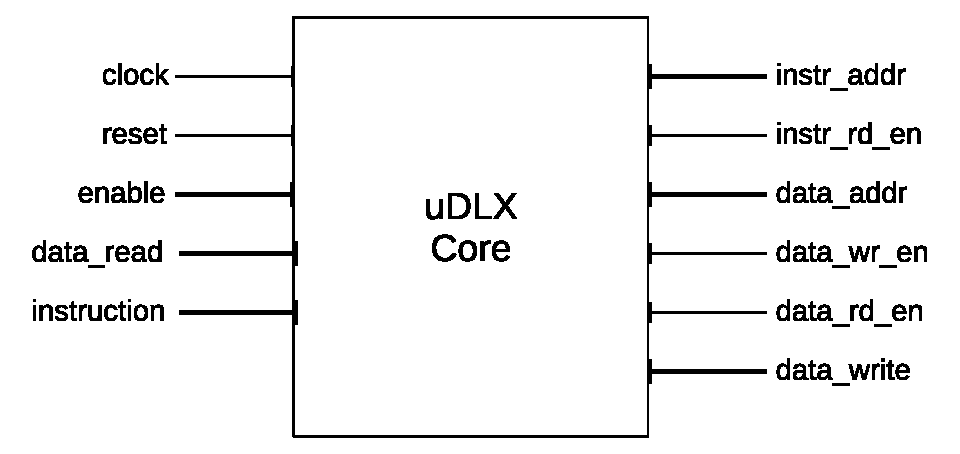
\includegraphics[width=.8\linewidth]{pictures/udlx_block.eps}
  \label{fig:datapath}
  \end{figure}
 
 
  \subsection{Pin/Port Definitions}
  \FloatBarrier
  \begin{table}[H]
    \begin{center}
      \begin{tabular}[pos]{| l | c | c | m{7cm} |} \hline 	
      \multicolumn{1}{|c|}{\cellcolor[gray]{0.9}\textbf{Name}} & 
      \multicolumn{1}{c|}{\cellcolor[gray]{0.9}\textbf{Length}} & 
      \multicolumn{1}{c|}{\cellcolor[gray]{0.9}\textbf{Direction}} &
      \multicolumn{1}{c|}{\cellcolor[gray]{0.9}\textbf{Description}} \\ \hline
	 clock 		& 1 	& input 	& CPU core clock  	\\ \hline
	 reset 		& 1	& input		& CPU core reset  	\\ \hline
	 sram\_data\_io 	& 16	& in/out 	& SRAM data \\ \hline
	 sdram\_data\_io 	& 32	& in/out 	& SDRAM data \\ \hline
	 sram\_addr 	& 20	& input 	& SRAM address \\ \hline
	 sram\_we\_n 	& 1	& output 	& SRAM write enable  \\ \hline
	 sram\_oe\_n 	& 1	& output 	& SRAM output enable  \\ \hline
	 sdram\_addr 	& 13	& in/out	& SDRAM address \\ \hline
	 sdram\_we 	& 1	& output 	& SDRAM write enable  \\ \hline
	 sdram\_oe 	& 1	& output 	& SDRAM output enable  \\ \hline
      \end{tabular}
    \end{center}
  \end{table}  
   
  \subsection{Parameters and Configurations}

 \FloatBarrier
  \begin{table}[H]
    \begin{center}
      \begin{tabular}[pos]{| l | l | m{8cm} |} \hline 	
      \multicolumn{1}{|c|}{\cellcolor[gray]{0.9}\textbf{Name}} & 
      \multicolumn{1}{c|}{\cellcolor[gray]{0.9}\textbf{Value}} & 
      \multicolumn{1}{c|}{\cellcolor[gray]{0.9}\textbf{Description}} \\ \hline
	  & &  	\\ \hline
      \end{tabular}
    \end{center}
  \end{table} 
    
  \newpage
  \section{Architecture Description}
  \label{sec:architecture_description}
  
  The data path developed to perform the synchronization is composed by:
  
  \subsection{Instructions Layout}
  
  \subsection{Functional Data Path Description}
  
  \subsubsection{Stage 1 - Instruction Fetch}
  
  \subsubsection{Stage 2 - Instruction Decoding}
  
  \subsubsection{Stage 3 - Execution}
  
  \subsubsection{Stage 4 - Memory}
  
  \subsubsection{Stage 5 - Write Back}
  
  \subsection{Pipeline Register Description}
  
  \subsection{Control Micro-instructions Description}
 
  %\newpage
  %\section{Timing}
    
% \bibliographystyle{ieeetr}
% \bibliography{ipprocess}

\end{document}
